% -------------------------------------------------------------------- %
% -------------------------------------------------------------------- %
% -------------------------------------------------------------------- %

\documentclass[twocolumn,10pt]{article} % here we use the article class, rather than elsarticle

% -------------------------------------------------------------------- %
% -------------------------------------------------------------------- %
% -------------------------------------------------------------------- %

\usepackage[square,numbers,sort&compress,comma]{natbib}

\usepackage{amsmath}
\usepackage{amssymb}
\usepackage{xcolor}
\usepackage{caption}
\usepackage{graphicx}
\usepackage{latexsym}
\usepackage{times}
\usepackage{dblfloatfix}

% -------------------------------------------------------------------- %
% -------------------------------------------------------------------- %
% -------------------------------------------------------------------- %

\topmargin - 12pt % might need to be set to 0pt for some installations
\oddsidemargin 32pt
\textheight 610pt
\textwidth 408pt
\columnsep 24pt

% -------------------------------------------------------------------- %
% -------------------------------------------------------------------- %
% -------------------------------------------------------------------- %

\def\thepage{}

\renewenvironment{abstract}%
              {% - begin definition
               \small% - select font
               {\bfseries \abstractname}% - select font
               \par% - end a paragraph (skip \parsep)
               \vspace{10pt}% - add vertical space
              }% - complete definition

\renewcommand\abstractname{Abstract}

\newcommand{\nomenclature}% - name of command
              [1]% - number of arguments
              {% - begin definition
               \bgroup% - begin a local group
               \flushleft% - turn on flushleft option
               \small\bf% - select font
               #1% - insert title text
               \par% - end a paragraph (skip \parsep)
               \egroup% - terminate local group
              }% - complete definition

\renewcommand{\section}% - name of command
              [1]% - number of arguments
              {% - begin definition
               \bgroup% - begin a local group
               \flushleft% - turn on flushleft option
               \small\bf% - select font
               \stepcounter{section}% - increment counter
               \arabic{section}. #1% - insert title text
               \par% - end a paragraph (skip \parsep)
               \egroup% - terminate local group
              }% - complete definition

\renewcommand{\subsection}% - name of command
              [1]% - number of arguments
              {% - begin definition
               \bgroup% - begin a local group
               \flushleft% - turn on flushleft option
               \small\em% - select font
               \stepcounter{subsection}% - increment counter
               \arabic{section}.% - insert title text
               \arabic{subsection}. #1% - insert title text
               \par% - end a paragraph (skip \parsep)
               \egroup% - terminate local group
              }% - complete definition

\renewcommand{\subsubsection}% - name of command
              [1]% - number of arguments
              {% - begin definition
               \bgroup% - begin a local group
               \flushleft% - turn on flushleft option
               \small\em% - select font
               \stepcounter{subsubsection}% - increment counter
               \arabic{section}.% - insert title text
               \arabic{subsection}.% - insert title text
               \arabic{subsubsection}. #1% - insert title text
               \par% - end a paragraph (skip \parsep)
               \egroup% - terminate local group
              }% - complete definition

  \newcommand{\acknowledgement}% - name of command
              [1]% - number of arguments
              {% - begin definition
               \bgroup% - begin a local group
               \flushleft% - turn on flushleft option
               \small\bf% - select font
               #1% - insert title text
               \par% - end a paragraph (skip \parsep)
               \egroup% - terminate local group
              }% - complete definition

  \newcommand{\sectionbib}% - name of command
              [1]% - number of arguments
              {% - begin definition
               \bgroup% - begin a local group
               \flushleft% - turn on flushleft option
               \small\bf% - select font
               #1% - insert title text
               \par% - end a paragraph (skip \parsep)
               \egroup% - terminate local group
              }% - complete definition

\renewcommand\figurename{Fig.}
\renewcommand{\captionsize}{\footnotesize}
\setlength\abovecaptionskip{0pt}
\setlength\belowcaptionskip{0pt}

\renewcommand\bibsection{\sectionbib{\refname}}

\setlength\bibsep{0pt}

\pagenumbering{arabic}

% -------------------------------------------------------------------- %
% -------------------------------------------------------------------- %
% -------------------------------------------------------------------- %

\begin{document}

\title{\LARGE Mitigation of thermoacoustic instability in \\
                     a turbulent combustor via self-coupling}

\author{{\large Ankit Sahay$^{*}$, Author 2 full name$$, Author 3 full name$$, $\ldots$ (13/15)}\\[10pt]
        {\footnotesize \em $^a$Indian Institute of Technology Madras, Chennai 600036, India }\\[-5pt]}

\date{}

% -------------------------------------------------------------------- %
% -------------------------------------------------------------------- %
% -------------------------------------------------------------------- %

\small
\baselineskip 10pt

% -------------------------------------------------------------------- %
% -------------------------------------------------------------------- %
% -------------------------------------------------------------------- %

\twocolumn[\begin{@twocolumnfalse}
\vspace{50pt}
\maketitle
\vspace{40pt}
\rule{\textwidth}{0.5pt}
\begin{abstract} % 100 to 300 words.
%
In this paper, we report the first observation of complete suppression of thermoacoustic instability in a bluff-body stabilized turbulent combustor through the method of self-coupling. Such self-coupling is achieved by mutually coupling the acoustic field of the combustor to itself through a single coupling tube. We characterize the effects of such acoustic self-feedback on the dynamical behavior of the system for the variation of different parameters of the coupling tube. We observe that the amplitude of acoustic pressure fluctuations quenched gradually as the length of the coupling tube is increased to an optimal range. The dynamical behavior of these oscillations changes from limit cycle to chaos via intermittency. % Chaos is observed during the state of complete suppression of acoustic pressure oscillations in the combustor.
We also study the coupled behavior of the acoustic field and the unsteady flame dynamics in the turbulent combustor. As the combustor approaches the state of complete suppression, the temporal synchrony between the acoustic pressure and heat release rate signals changes from the state of synchronized periodicity to desynchronized chaos through intermittent synchronization. Finally, we compare the change in the spatiotemporal distribution of acoustic power in the combustor during the mitigation of thermoacoustic instability. We notice the complete disruption of the coherent spatial structures of acoustic energy production observed during the state of thermoacoustic instability, as these instabilities are suppressed through self-coupling in the combustor. Thus, we anticipate acoustic self-feedback after appropriate time delay to be a viable option to mitigate high amplitude thermoacoustic oscillations in turbulent combustion systems present in gas turbines and rocket engines. 
%
\end{abstract}
\vspace{10pt}
\parbox{1.0\textwidth}{\footnotesize {\em Keywords:} Thermoacoustic instability; self-coupling; acoustic feedback}
\rule{\textwidth}{0.5pt}
\vspace{10pt}
\end{@twocolumnfalse}] 

% -------------------------------------------------------------------- %
% -------------------------------------------------------------------- %
% -------------------------------------------------------------------- %

\clearpage

\section{Introduction} \addvspace{10pt}

Thermoacoustic instabilities have proven to be a major deterrence to the development of low-emission gas turbine engines used for power generation and propulsion applications \cite{lieuwen2005combustion}. These are ruinously large amplitude pressure oscillations  established in gas turbine engines and similar systems when a positive feedback is developed between the acoustic field and the heat release rate fluctuations in the reaction field of the combustor \cite{sujith2021thermoacoustic}. The presence of such instabilities results in serious performance losses, structural degradation due to increased heat transfer and reduced operational range \cite{culick1991combustion}. As a result of potential harm to the structural integrity of a system, it is necessary to find ways to mitigate thermoacoustic instabilities in the course of developing a new dynamically stable combustion systems.

Traditionally, different mechanisms of closed-loop and open-loop active controls (i.e., feedback control or external forcing, respectively) have been developed as a viable way of suppressing thermoacoustic instability \cite{ mcmanus1993review, dowling2005feedback}. However, these methods suffer from several limitations such as the use of complex electro-mechanical components, lack of reliability of sensors for operating in the harsh environment of practical combustors, high maintenance and replacement costs, and high power requirements for operating feedback control units. Another way to mitigate combustion instabilities is to use passive damping devices such as Helmholtz resonators \cite{dupere2005use}, quarter-wave resonator \cite{park2010nonlinear}, half-wave resonators \cite{park2009optimal}, and Herschel-Quincke tubes \cite{park2008thermo}, which have shown promising performance in suppressing thermoacoustic instability in many lab-scale and practical combustors \cite{bellucci2004use}. However, passive control strategies involve limited range of operation and the testing of passive controls on actual hardware of the combustor is cumbersome and expensive. 

%A combustor exhibiting self-sustained limit cycle oscillations (LCO) can be considered as a nonlinear oscillator. 
Recently, a method from synchronization theory called mutual coupling of oscillators has been adopted to suppress thermoacoustic instabilities in two systems \cite{sujith2021thermoacoustic}. At appropriate coupling parameters, the dynamical behavior of both the systems approach the same steady state, known as amplitude death in nonlinear dynamics parlance \cite{zou2021quenching}. Through experimental and numerical approaches, a few studies have extensively investigated the presence of amplitude death and partial amplitude death in coupled laminar thermoacoustic systems \cite{thomas2018effect, dange2019oscillation, sahay2021dynamics, srikanth2021dynamical, hyodo2020suppression}. In addition, some studies have investigated the dynamics of mutually coupled turbulent flame-driven turbulent combustors \cite{jegal2019mutual, moon2020mutual, guan2021low}, and have also reported the presence of amplitude death in them \cite{jegal2019mutual}. The mutual coupling between the systems is achieved by using a single or double tubes of fixed lengths and diameters. An increase in the length of the coupling tube correspondingly increases the delay time in the coupling of acoustic field in the systems, while increase in the diameter of the tube increases the strength of coupling between the systems \cite{dange2019oscillation, sahay2021dynamics}. Thus, these studies demonstrate the effectiveness of mutual coupling in suppressing thermoacoustic instabilities in two or more systems. 

In contrast to the aforementioned studies, in this paper, we present the first application of the method of mutual coupling, known as self-acoustic delayed feedback, to suppress thermoacoustic instabilities in a single turbulent combustion system. Here, the self-feedback is achieved by coupling the acoustic field of the combustor to itself, after a finite time delay, through a coupling tube of a specific length and diameter. This method has recently been used by a few researchers to suppress limit cycle oscillations in the acoustic field of different laminar systems such as electro-acoustic system \cite{biwa2016suppression}, acoustic pipeline \cite{lato2019passive}, and horizontal Rijke tube \cite{srikanth2021selfcoupling}. These studies have shown that self-coupling affects the bifurcation characteristics of a single system \cite{srikanth2021selfcoupling}, where the suppression of acoustic pressure oscillations is realized only when a tube of a length equal to the odd multiple of the half-wavelength of the anticipated acoustic standing wave is used \cite{biwa2016suppression, lato2019passive}. %, and by Lato et al. \cite{lato2019passive} on acoustic pipelines, showed that maximum suppression is realized only when a tube with a length equal to the odd integer times the half wavelength of the anticipated acoustic mode is used for self-coupling. Srikanth et al. {\textbf{(Ref)}} were the first to completely suppress thermoacoustic instability by inducing self-coupling in a horizontal Rijke tube.
Although these studies provide an understanding of the changes that happen in the acoustic field during mitigation of limit cycle oscillations in a self-coupled laminar system, this information might be insufficient to predict the suppression of thermoacoustic instabilities in turbulent combustion systems. 

We know that thermoacoustic instabilities are a result of the complex interaction between the flow, the flame, and the acoustic field of a combustor \cite{sujith2021thermoacoustic}. As per the Rayleigh criterion, such instabilities occur only when in-phase synchrony is developed between the acoustic pressure and heat release rate fluctuations in the combustor \cite{rayleigh1878explanation}. Since the coupling between these subsystems plays an important role in the genesis of thermoacoustic instabilities, it is important to understand how the temporal and spatiotemporal coupling between these subsystems change during the suppression of thermoacoustic instability when the system is self-coupled. Towards this purpose, we systematically address the following questions in this paper - (i) can we mitigate thermoacoustic instability via self-coupling in a turbulent combustor? (ii) what is the nature of the transition of acoustic pressure fluctuations during the suppression of thermoacoustic instability? and (iii) how does the temporal and spatiotemporal coupling between the acoustic pressure and heat release rate oscillations get affected due to self-coupling? 
\begin{figure*}[t]
\centering
\includegraphics[width=1\textwidth]{fig1.pdf}
\caption{The schematic of a turbulent bluff-body stabilized dump combustor subjected to self-coupling using a single connecting tube.}
\label{TARA_fig}
\end{figure*}

We performed experiments on a laboratory-scale bluff body stabilized turbulent combustor. We report the complete suppression of thermoacoustic instability in the combustor through the method of delayed acoustic self-feedback applied through a coupling tube. We found that, as the length of the coupling tube is changed, the amplitude and the frequency of acoustic pressure fluctuations exhibit a gradual decrease, and their dynamical behavior display a transition from the state of limit cycle oscillations to chaos via intermittency. We observe a lack of suppression of thermoacoustic instabilities when their amplitude prior to coupling is above a critical value, for fixed parameters of the coupling tube. We also notice a gradual decay in the temporal synchrony between the acoustic pressure and the heat release rate fluctuations as the system dynamics approaches the complete state of suppression. Finally, we notice that the coherent regions of acoustic power production, observed due to local synchrony between the acoustic pressure fluctuations and the heat release rate fluctuations in the spatial field of the combustor, inhibits during the transition to complete suppression of thermoacoustic instability.

\section{Experimental Setup} \addvspace{10pt}

We perform experiments of self-coupling on a turbulent bluff-body stabilized dump combustor at ambient operating conditions (Fig.~\ref{TARA_fig}). The combustor has a rectangular cross-section of $ 90 \times 90$ $\text{mm}^2$ and a length of $1060$ $\text{mm}$. The experimental setup consists of a plenum chamber, a burner, a combustor, and an extended duct. Air first enters the plenum chamber to ensure that the flow entering the systems is immune from the upstream disturbances. The air and the fuel (Liquefied Petroleum Gas, 60\% butane and 40\% propane) are partially mixed in the burner section before entering the main combustion chamber. Air and fuel flow rates are controlled through mass flow controllers (Alicat Scientific, MCR series) and have a measurement uncertainty of $\pm$ ($0.8 \%$ of reading + $0.2\%$ of full-scale). During experiments, we fix the fuel flow rate ($\dot{m_f}$) at a fixed value and vary the air flow rate ($\dot{m_a}$) to establish thermoacoustic instability in the combustor. The Reynolds number of air flow rate is varied in the range of 14300-24500. We use a spark plug to ignite the partially premixed air fuel mixture at the dump plane using a 11 kV ignition transformer. A circular disk of thickness 10 mm and diameter 47 mm is used as the flame holding device. This bluff-body is positioned at 30 mm downstream of the dump plane. The combustion products are exhausted through a long duct into the atmosphere. 

Self-coupling is established in the combustor by acoustically coupling the combustor to itself using a single stainless steel flexible braided tube of different lengths $L_c$ and internal diameters $d$. The self-coupling tube is attached to two opposite sides of the combustor walls at an axial distance of 10 cm from the dump plane (refer to Fig.~\ref{TARA_fig}).  Ball-type valves are manually operated to switch on and off the self-coupling of the acoustic fluctuations in the system. During self-coupling experiments, we first establish thermoacoustic instability of particular amplitude in the system and then switch on the coupling by opening the valve. The amplitude of acoustic pressure fluctuations during thermoacoustic instability is primarily varied by changing the fuel flow rate in the system.  

The acoustic pressure measurements in the system, at different conditions of coupling and operating parameters, are performed using a PCB103B02 piezoelectric transducer (sensitivity: 217 mV/kPa and uncertainty: $\pm$0.15 Pa) mounted on the combustor wall at 20 mm from the dump plane. A photomultiplier tube (PMT, Hamamatsu H10722-01) equipped with a CH* filter (wavelength of 430 nm and 12 nm FWHM) module is used to capture the global heat release rate fluctuations in the flame ($\dot{q}^\prime$). We simultaneously acquired the data of both the acoustic pressure and the global heat release rate signals for a duration of 3 s at a sampling rate of 10 kHz using an A/D card (NI-6143, 16 bit). High-speed CH* chemiluminescence images of the flame are simultaneously captured with acoustic pressure fluctuations at 2000 fps for 3 s using a CMOS camera (Phantom - V12.1 with a ZEISS 50 mm camera lens). The flow-field spanning 90 mm $\times$ 120 mm at a resolution of 574 $\times$ 764 pixels is imaged from the dump plane. 


\section{Results and Discussion} \addvspace{10pt}

In this section, we systematically present the effect of self acoustic feedback through a single coupling tube on the suppression characteristics of thermoacoustic instability in a turbulent combustor. We observe a significant change in the dynamics of acoustic pressure fluctuations when the combustor is self-coupled in a particular range of the length and diameter of the coupling tube. At optimum values of these coupling tube parameters, we were able to completely suppress thermoacoustic instability just by coupling the acoustic field of the system to itself after a finite time delay, corresponding to the length of the coupling tube, without any prepossessing of the acoustic signal as done in the traditional active closed-loop controls. We will first discuss temporal changes happening in the acoustic pressure signal and then present changes happening in the coupled behavior of acoustic pressure and heat release rate fluctuations of the system, during the mitigation of thermoacoustic instability via the method of self-coupling.  

% \textcolor{red}{In this section, we will first discuss the dynamics of these fluctuations during the route to suppression of thermoacoustic instability and then will examine the temporal and spatiotemporal changes happening in the coupled behavior of acoustic pressure and heat release rate fluctuations of the system during this route.} 

\subsection{Route from thermoacoustic instability to the state of complete suppression} \addvspace{10pt}

In Fig. \ref{fig2}, we show the percentage change in the root-mean-square (RMS) value of acoustic pressure fluctuations $\Delta p^\prime_{rms}$ as a function of the lengths of the coupling tube, when the the internal diameter of the coupling tubes are kept constant at 2.54 cm. $\Delta p^\prime_{rms}$ is calculated as the difference between the values during the state of thermoacoustic instability (in an uncoupled state, $p^\prime_{rms0}$) and during the state of self-coupling ($p^\prime_{rms}$), i.e., $\Delta p^\prime_{rms} = p^\prime_{rms0}-p^\prime_{rms}$. The value of $\Delta p^\prime_{rms}$ is further normalized by the difference in the RMS values of acoustic pressure fluctuations observed during the state of combustion noise and thermoacoustic instability ($p^\prime_{rms(\text{TAI-CN})}$). %The horizontal axes shows the absolute length of the coupling tube (in cm), and the normalized length as a fraction of the combustor length ($L_{duct} = 1060$ cm). 
%Experiments are performed to investigate the changes in the nature of the acoustic pressure fluctuations when the length of the coupling tube ($L_c$) is increased as the control parameter. For all the experiments, the internal diameter of the coupling tubes are kept constant at 2.54 cm. 
In the figure, the blue, red, and green shaded intervals denote the regions where the intermediate suppression, complete suppression, and no suppression, respectively, of thermoacoustic instability observed ($p^\prime_{rms}  \approx 3200$ Pa) after self-coupling is induced in the combustor. We notice a gradual decrease in the amplitude of thermoacoustic instability during the occurrence of complete suppression as $L_c$ is increased. However, post the region of suppression at higher values of $L_c$, the amplitude thermoacoustic instability remains nearly the same. 

\begin{figure}[t]
\centering
\includegraphics[width=192pt]{fig2.png}
\caption{The variation of $p^\prime_{rms}$ (normalized) of self-coupled combustor with respect to the absolute ($L_c$ on bottom axis) and normalized ($L_c/L_{duct}$ on top axis) length of the coupling tube. $L_{duct} = 1060$ cm denotes the length of the combustor. The internal diameter of the coupling tube is maintained at $d=2.54$ cm. }
\label{fig2}
\end{figure}

 Figure ~\ref{fig3} shows the change in the characteristics of acoustic pressure fluctuations, plotted in terms of time series, power spectrum, and scalogram, in the absence of coupling (Fig.~\ref{fig3}a) and when the system is self-coupled for different lengths of the coupling tube (Fig.~\ref{fig3}b-e). In the absence of self-coupling, during thermoacoustic instability (Fig.~\ref{fig3}a), we observe large amplitude periodic oscillations in the the time series (Fig.~\ref{fig3}a-i), a sharp spectral peak at 163.9 Hz corresponding to the fundamental mode of the combustor in the power spectrum (Fig.~\ref{fig3}a-ii), and a continuous distribution of the spectral power throughout time in a narrow frequency band in the scalogram (Fig.~\ref{fig3}a-iii).

\begin{figure*}[t!]
\centering
\includegraphics[width=1\textwidth]{fig3.png}
\caption{Variation of (i) time series, (ii) power spectral density, and (iii) scalograms of acoustic pressure fluctuations $p^\prime$ as the turbulent combustor transitions from a state of (a) thermoacoustic instability to (b-e) complete suppression of oscillations via intermittency.}
\label{fig3}
\end{figure*}

As soon as the self acoustic feedback is established via a coupling tube, we notice a change in the dynamical properties of acoustic pressure fluctuations in the system. We found that the suppression of thermoacoustic instability with an increase in $L_c$ is associated with the change in its dynamical behavior from large amplitude periodic oscillations (Fig.~\ref{fig3}b) to low amplitude chaotic oscillations in the state of complete suppression (Fig.~\ref{fig3}e) via the state of intermittent oscillations (Fig.~\ref{fig3}c,d). During intermittent oscillations, regions of low amplitude chaotic fluctuations separates regions of large amplitude periodic oscillations in an apparently random manner (see insets in Fig.~\ref{fig3}d). The existence of chaos during the state of complete suppression of thermoacoustic instability is confirmed from the widely accepted 0-1 test of chaos \cite{gottwald2004new}. The results of the 0-1 test of chaos are presented in Supplementary Material due to the space constraint. 

We notice a gradual shift in the dominant frequency of periodic oscillations towards a lower value in the power spectrum of acoustic pressure fluctuations during the suppression of thermoacoustic instability (compare plots in Fig.~\ref{fig3}a-ii to Fig.~\ref{fig3}e-ii). The scalogram plots during this transition show an increase in interruptions in the dominant spectral power of the signal (Fig.~\ref{fig3}b-iii to Fig.~\ref{fig3}d-iii) and is nearly disappeared during the state of complete suppression of thermoacoustic instability (Fig.~\ref{fig3}e-iii). Thus, we observe that the both the temporal and spectral properties of acoustic pressure fluctuations exhibit a gradual change during the mitigation of thermoacoustic instability in a self-coupled turbulent combustor. %This behavior of the self-coupled turbulent system shows a qualitative similarity with that observed in the model of mutually coupled two Rijke tube systems in the presence of noise by Thomas \textit{et al.} \cite{thomas2018effect1}. %According to them, the gradual transition during the suppression of oscillations happens due to amplification of the  of 


%For low values of the self-coupling tube length, i.e. $L_c = 120$ cm, the self-coupled combustor exhibits periodic oscillations with small intervals of aperiodicity. This can be confirmed by the increase in the broadband nature of the frequency spectrum (Fig.~\ref{fig3}b-ii) compared to that for the state of thermoacoustic instability (Fig.~\ref{fig3}a-ii). The intervals exhibiting aperiodic oscillations can be clearly seen from the breaks in the dominant spectral power band observed in the corresponding scalogram (Fig.~\ref{fig3}b-iii). As the length of the coupling tube is increased to higher values, i.e. 130 cm and 140 cm, we observe a gradual decrease in the amplitude of the acoustic pressure fluctuations, a decrease in the dominant frequency visible in the power spectrum, and a broadening of the power spectrum around the dominant frequency. 

%We observe the state of intermittency when a coupling tube length $L_c = 140$ cm is used to self-couple the combustor. In Fig. ~\ref{fig3}d-i, we notice the occurrence of bursts of periodic oscillations in between regions of low amplitude aperiodic oscillations in an apparently random manner (see inset of Fig.~\ref{fig3}d). During this state, the power spectrum shows the existence of multiple spectral peaks in Fig.~\ref{fig3}d-ii. The presence of intermittent oscillations is also confirmed from the occurrence of intermittent breaks observed around the dominant frequency band in the scalogram (Fig.~\ref{fig3}d-iii).

%As the length of the coupling tube length is increased to $L_c = 160$ cm, we transition to the state of a completely suppressed state, where the combustor exhibits a completely aperiodic signal (Fig.~\ref{fig3}e-i). During the state of complete suppression, we notice an apparently random distribution of the spectral power in the scalogram (Fig.~\ref{fig3}e-ii), indicating the absence of a distinct common frequency in the acoustic pressure oscillations. The existence of chaos during the state of complete suppression is confirmed from the 0-1 test of chaos (See Supplementary Material). Thus, the system dynamics change its behavior from a state of periodic oscillations, observed during thermoacoustic instability, to the chaotic state, observed during the state of complete suppression, through the occurrence of intermittent bursts of periodic oscillations.

\subsection{Temporal analysis of coupled acoustic pressure and global heat
release rate fluctuations}

Now, we investigate the change in the coupled interaction between the acoustic pressure ($p^\prime$) and the heat release rate ($\dot{q}^\prime$) fluctuations during the suppression of thermoacoustic instability, by examining the locking of their instantaneous phases and frequencies (Fig.~\ref{fig4}). The time-frequency locking (i.e., synchronization) of such signals can be analyzed using a cross wavelet transform plot \cite{grinsted2004application, pawar2019temporal}. In this plot, the regions of common spectral power for both the signals in time are highlighted by a brighter color and the corresponding wrapped instantaneous relative phase between them are indicated by arrows. When the signals are synchronized in time, their cross wavelet transform shows a larger magnitude of the spectral power throughout the signal and a constant alignment of arrows at a particular phase difference. In contrast, desynchronization of signals is indicated in the cross wavelet transform plot by a near random distribution of the common spectral power and an arbitrary alignment of arrows in time. % In Fig.~\ref{fig4}, we plot the acoustic pressure and heat release rate fluctuations for different lengths of the coupling tube, along with the corresponding cross wavelet transforms computed between the two signals. A black thin line at the bottom of each cross-wavelet transform plot represents the region of the 'cone of influence' \cite{grinsted2004application}.

\begin{figure*}[t!]
\centering
\includegraphics[width=0.9\textwidth]{all_copy.png}
\caption{Cross wavelet transform plots between $p^\prime$ and $\dot{q}^\prime$ signals and the temporal variation of their phase difference associated with the dominant frequency (indicated by a red dotted line and an arrow on the left of each cross wavelet transform plot), during (a) the state of thermoacoustic instability in the absence of self-coupling and (b-d) for the states of self-coupled combustor with increasing length of the coupling tubes. The internal diameter of the coupling tubes is kept constant at 2.54 cm. }
\label{fig4}
\end{figure*}

\begin{table*}[!b] \small
\centering
\caption{\label{table} Phase Locking Value (PLV) and Pearson's Correlation Coefficient ($\rho$) between $p^\prime$ and $\dot{q}^\prime$ for different $L_c$.}
\begin{tabular}{|l|l|l|l|l|l|l|l|l|l|l|l|l|}
\hline
$L_c$ (in cm)                   & 100  & 110  & 120  & 130  & 140  & 150  & 160  & 170  & 180  & 190  & 200  & 215  \\
\hline
PLV                 & 0.97 & 0.96 & 0.91 & 0.84 &   -   &    -  &   -   & 0.94 & 0.93 & 0.95 & 0.91 & 0.93 \\
\hline
$\rho$ & 0.64 & 0.62 & 0.65 & 0.60 & 0.41 & 0.37 & 0.25 & 0.55 & 0.55 & 0.69 & 0.64 & 0.59 \\
\hline
\end{tabular}
\label{table}
\end{table*}


In Fig. \ref{fig4}a, we notice that both $p^\prime$ and $\dot{q}^\prime$ signals are perfectly synchronized at a frequency of 163.9 Hz, where the relative phase ($\Delta\phi$) between them stays constant around 35.3 deg. When the system is self-coupled for $L_c = 120$ cm, in the regime of intermediate suppression of $p^\prime$ oscillations (Fig. \ref{fig2}), we observe the appearance of a common frequency band around the dominant frequency of 131.5 Hz, for almost the entire length of the signal (Fig.~\ref{fig4}b). The instantaneous phase difference ($\Delta\phi$) plot at 131.5 Hz is nearly constant around a mean value of 42.7 deg throughout the signal except a small phase jump at a particular time instance, which happens when the signals are locally desynchronized at that particular instant. As the length of the coupling tube $L_c$ is increased to higher values of 140 and 160 cm (Fig.~\ref{fig4}c and Fig.~\ref{fig4}d, respectively), we notice a corresponding increase in the discontinuities in the occurrence of common frequency bands of these signals in the cross wavelet transform plots. This increase in discontinuities of frequency synchronized regions of the signals in the cross wavelet transform plot can be easily seen from the plots of $\Delta\phi$, where we notice an increase in the number of phase jumps about a mean phase difference for these signals. This behavior of the temporal variation of $\Delta\phi$ can be associate with the increase in the duration of desynchronization of $p^\prime$ and $\dot{q}^\prime$ oscillations in the system. We found that these instances of desynchronized oscillations corroborate with the occurrence of low amplitude chaotic oscillations in $p^\prime$ and $\dot{q}^\prime$ signals. During the state of suppression of thermoacoustic instability (for $L_c = 160$ cm in Fig. \ref{fig4}d), we notice desynchronization of $p^\prime$ and $\dot{q}^\prime$ signals in the system. This happens when a sustained positive feedback between these oscillations is completely vanished. 

Thus, we observe that the synchronization behavior of coupled $p^\prime$ and $\dot{q}^\prime$ signals gradually decreases during the mitigation of thermoacoustic instability as $L_c$ is increased. In other words, suppression of thermoacoustic instability in a turbulent combustor is associated with the change in the coupled behavior of $p^\prime$ and $\dot{q}^\prime$ oscillations from synchronized periodicity to desynchronized chaos via intermittent synchronized oscillations.  


%During the regime of intermediate suppression of acoustic pressure oscillations (i.e., for $L_c = 120$ cm), we observe the appearance of a common frequency band around the dominant frequency of 131.5 Hz of the pressure and heat release rate signals, for almost the entire length of the signal in Fig.~\ref{fig4}a. The indicates synchronization these signals at this condition of self-coupling in the system. The mean phase difference of these synchronized oscillations is around AA deg. A few breaks observed in the common frequency band are the result of the presence of desynchronization of these signals. These desynchronized regions corroborate with low amplitude chaotic oscillations observed in the system. As the length of the coupling tube $L_c$ is increased to higher values of 130 and 140 cm (Fig.~\ref{fig4}b and Fig.~\ref{fig4}c, respectively), we notice a corresponding increase in the duration of desynchronized oscillations between the synchronized regions of the signals, which can be confirmed from the increased number of discontinuities observed in the common frequency band of the respective cross wavelet transform plots. This is similar to the existence of intermittent synchronization between the acoustic pressure and heat release rate oscillations.
%During intermittency observed in Fig~\ref{fig4}c, we observe the regions of enhanced coupling between the acoustic pressure and the heat release rate fluctuations, mostly during epochs of bursts of periodic oscillations. The existence of such a short-term coupling results in the intermittent occurrence of regions of common frequency between the acoustic pressure and heat release rate signals. The presence of alternating epochs of periodic and aperiodic signals during intermittency cab be seen in the inset in Fig.~\ref{fig4}c. 


%During the state of complete suppression of thermoacoustic instability (for $L_c = 160$ cm), we notice an apparently random distribution of the spectral power in the common frequency region of the cross wavelet transform plot (Fig.~\ref{fig4}d), indicating the absence of a distinct common frequency in both the acoustic pressure and heat release rate fluctuations. The presence of a large extent of discontinuities in the common frequency band indicates the significant lack of synchrony between these in the system. Thus, we observe that the synchronization behavior of coupled acoustic pressure and heat release signals diminishes during the suppression of thermoacoustic instability. In the absence of any sustained positive feedback between these oscillations, observed in the form of complete desynchrony, thermoacoustic instabilities are suppressed in the system.

\begin{figure*}[t]
\centering
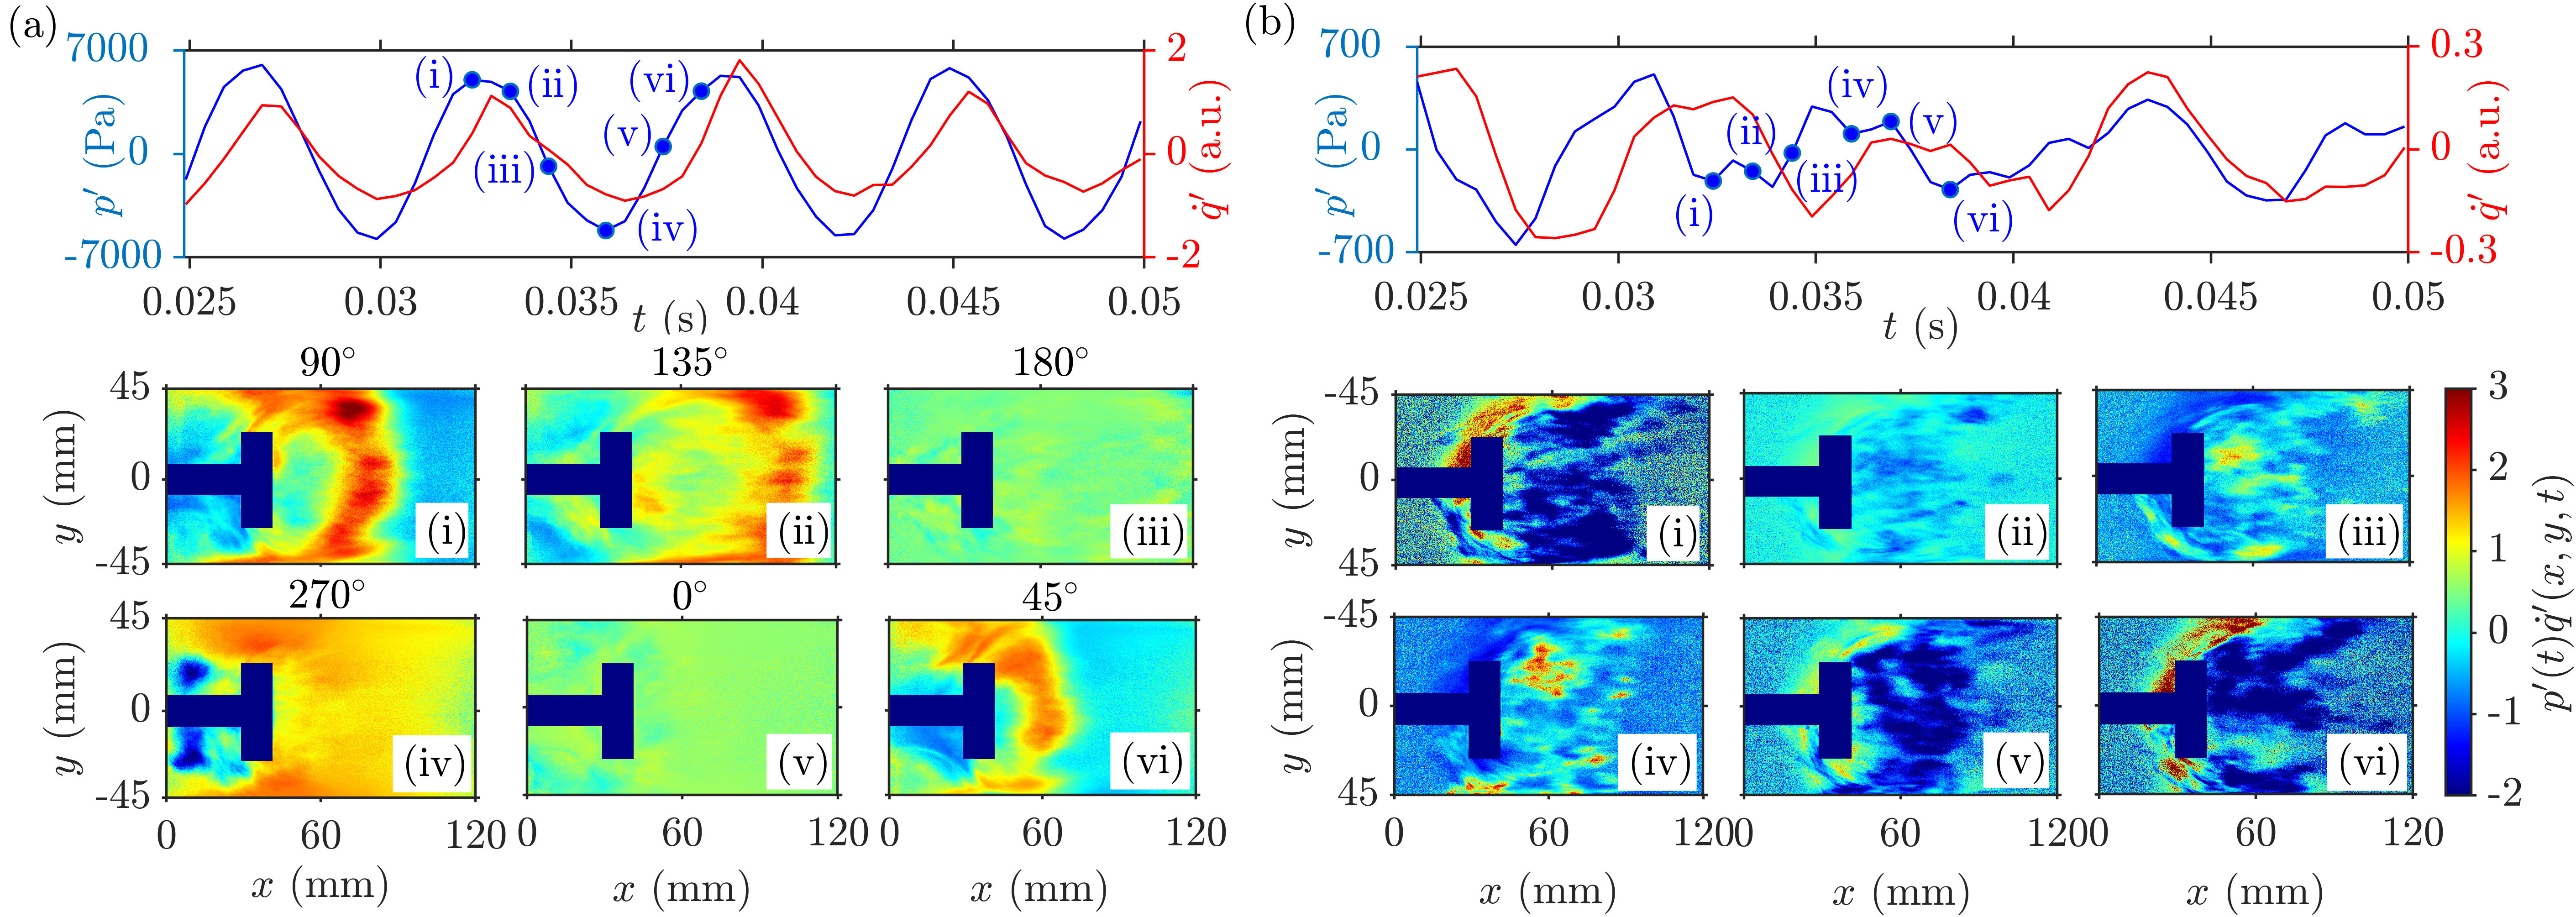
\includegraphics[width=1\textwidth]{spatio_temporal_5.png}
\caption{(a,b) Time series of $p^{\prime}(t)$ and $\dot{q}^{\prime}(t)$, (i-viii) phase-averaged and instantaneous distribution of $p^\prime(t)\dot{q}^\prime(x,y,t)$ during the states of (a) thermoacoustic instability, and (b) during complete suppression of oscillations in the turbulent combustor, respectively.}
\label{fig5}
\end{figure*}


In addition, we use two quantifiers, called phase locking value (PLV) and Pearson's Correlation Coefficient ($\rho$), to detect the synchronization behavior of $p^\prime$ and $\dot{q}^\prime$ signals as $L_c$ is varied across the region of suppression of thermoacoustic instability shown in Fig. \ref{fig2}. PLV helps us detect phase-synchronization and is calculated as $PLV = \dfrac{1}{N} \Bigg{\lvert} \sum\limits_{n=1}^N \text{exp}(i \Delta \phi) \Bigg{\lvert}$ \cite{pikovsky2001universal}. On the other hand, $\rho$ aids in finding amplitude correlation between the signals \cite{gonzalez2002amplitude} and is obtained as ADD Formula. We have presented the values of these measures in Table \ref{table}. We found that in the regime of intermediate suppression of thermoacoustic instability, both $p^\prime$ and $\dot{q}^\prime$ are phase synchronized, confirmed from the PLV near 1. Inside the regime of suppression, as the signals are aperiodic where the phase of the oscillations is not physically defined, we do not calculate PLV \cite{pikovsky2001universal,sujith2021thermoacoustic}. The value of $\rho$ is observed to be high positive value between 0.55 and 0.7 in the regime of thermoacoustic instability, while it drops to a lower value of 0.25 in the suppression region due to the lack of amplitude correlation between the signal.   



%We also investigate the amplitude correlation \cite{gonzalez2002amplitude} between the $p^\prime$ and $\dot{q}^\prime$ signals by calculating a linear measure of correlation, known as Pearson's Correlation Coefficient ($\rho)$, between these signals, as $L_c$ is varied across the region of suppression of thermoacoustic instability (Table \ref{table}). %We use Pearson's Correlation Coefficient ($\rho)$ to measure of the strength of the linear relation between the two signals. It further helps in determining the synchronization of amplitudes of the signals . 
%The values of $\rho$ range from $-1 $ to $+1$; $\rho = -1$ corresponds to strong negative correlation and $\rho = 1$ corresponds to strong positive correlation between the signals. %The value $\rho = 0$ indicates zero linear correlation between the signals. 
%We observe the value of $\rho$ around 0.6 in the regime where the signals are frequency (and also phase) synchronized for a longer duration in time, while its value is low when they are desynchrnized in regime of suppression.   
%In our system, we observe values of $\rho$ greater than zero, corroborating the presence of a positive correlation between the acoustic pressure and heat release rate oscillations. We notice an decrease in the value of the linear correlation as the system dynamics transitions from the state of intermediate suppression of oscillations to a state of complete suppression of oscillations. \textcolor{blue}{As the length of the coupling tube $L_c$ is increased beyond the region of maximum suppression ($L_c \geq 170$ cm in table \ref{table}), the magnitude of suppression of oscillations drops down to very low values ($\Delta p^\prime_{rms} < 10\%$), which is accompanied by an increase in the $\rho$ values.}

%\textcolor{blue}{The corresponding Phase Locking Values (PLV) which are calculated using the analytic signal approach utilizing the Hilbert transform, quantifies the degree of synchronization between the $p^\prime$ and $\dot{q}^\prime$ signals \cite{pikovsky2001universal}. The trajectories in the analytic plane for $p^\prime$ and $\dot{q}^\prime$ during the state of maximum suppression ($140$ cm $\leq L_c \leq$ $160$ cm in Table \ref{table}) do not have a unique center of rotation, thus we cannot strictly interpret the computed phase using Hilbert Transform as instantaneous phase. The PLV and the corresponding $\rho$ values in Table \ref{table} indicate that the $p^\prime$ and $\dot{q}^\prime$ signals are  phase-locked and more correlated during the states of intermediate and no suppression, in comparison to the correlation during the state of complete suppression.  }


\subsection{Spatiotemporal analysis during the complete suppression of thermoacoustic instability} \addvspace{10pt}


In this section, we compare the spatiotemporal changes happening in the combustor as thermoacoustic instabilities are suppressed due to the method of self-acoustic feedback. During the state of thermoacoustic instability, we notice the periodic emergence of large-scale vortical structures from the dump plane of the combustor. These vortices impinge on both the side walls of the combustor and the bluff-body. The breaking of these vortices results in the fine scale mixing of the reactants and hot products, causing a large heat release release fluctuations in the system. In contrast, during the state of complete suppression of thermoacoustic instability, we observe the absence of any such large-scale vortex in the combustor, wherein the flame dynamics appears to be nearly the same at all time instances. 

In Fig. \ref{fig5}, we show the instantaneous fields of $p^\prime(t) \dot{q}^\prime(x,y,t)$ (i.e., local acoustic power) compared over a period of the oscillation for the state of thermoacoustic instability (Fig. \ref{fig5}a(i-vi)) and a few time instances of the completely suppressed state of the oscillations (Fig. \ref{fig5}b(i-vi)). %The data points corresponding to these images are marked in the time series shown in Figs. \ref{fig5}a,b, respectively. 
In this figure, the blue color represents the local acoustic power sinks ($p^\prime(t) \dot{q}^\prime(x,y,t)$ $<0$), whereas the red color represents the local acoustic power sources ($p^\prime(t) \dot{q}^\prime(x,y,t)$ $>0$). 


During the state of thermoacoustic instability (Fig. \ref{fig5}a), we observe larger coherent regions of  acoustic power production ($p^\prime\dot{q}^\prime>0$) on the top and the downstream of the bluff-body. The coherent regions begin to form across the bluff-body when the acoustic pressure is near its local minima (Fig. \ref{fig5}a-i). As the amplitude of $p^\prime$ approaches the local maximum value, we notice a growth in the clusters of local acoustic power sources mostly in the downstream of the bluff-body (Fig. \ref{fig5}a-ii). When the pressure amplitude reaches its local maximum, these clusters of $p^\prime\dot{q}^\prime>0$ merge and spread over a larger region of the reaction flow field (Fig. \ref{fig5}a-iii). As the pressure amplitude decays, the region of $p^\prime\dot{q}^\prime>0$ decreases in size and observed in the form of a few clusters (Fig. \ref{fig5}a-iv to \ref{fig5}a-vi). This behavior of local acoustic power fluctuations repeats qualitatively in a similar manner over each oscillation cycle.  %whose value coherent structure convects downstream (from time instants (i) to (ii) in Fig. \ref{fig5}a) it grows in size. The coherent structure impinges on the top wall of the combustor (see time instant (iii) in Fig. \ref{fig5}a), and breaks down into small fragmented clusters. Upon impingement, a spike occurs in the global heat release rate due to sudden increase in the fine scale mixing of the reactants and hot products. We observe large regions of local acoustic power sources during the downstream convection and impingement of these coherent structures. We associate this behavior to the larger driving compared to the damping of the system during the state of thermoacoustic instability.}

During the state of complete suppression of thermoacoustic instability (Fig. \ref{fig5}b(i-vi)), %shows the instantaneous fields of $p^\prime(t) \dot{q}^\prime(x,y,t)$ for the sate of complete suppression, when the turbulent combustor is coupled to itself through a duct of length $L_c = 160$ cm. 
we observe that the spatial distribution of $p^\prime\dot{q}^\prime$ is highly disordered (incoherent) and its value is observed near 0 in majority of the reaction field of the combustor. We notice that the self-acoustic coupling of the combustor using a coupling tube of particular length and diameter breaks the constructive interactions between the acoustic pressure and local heat release rate oscillations, which causes lesser driving from the heat release rate field to the acoustic field of the combustor. As a result, the suppression of thermoacoustic instability is observed in the system. %in Fig. \ref{fig5}b is due to the reduction in the constructive interactions between acoustic pressure oscillations and global heat release rate oscillations, causing a suppression of the periodic formation of the coherent flow structures in the combustor duct. Subsequently, the suppression of the coherent flow structures changes the distribution of the local heat release rate leading to the disruption of the regions of positive $p^\prime(t) \dot{q}^\prime(x,y,t)$ in the local acoustic power field.} 

%\textcolor{blue}{Finally, we examine the amplitude response of the self coupled combustor on the variation of the root-mean-square values of the thermoacoustic instability ($p^\prime_{0,rms}$). The length and internal diameter of the coupling tube are kept constant at 140 cm and 2.54 cm, respectively. These coupling parameters are fixed in accordance with the results seen in Fig. \ref{fig2}, where we observe complete suppression of thermoacoustic instability for the aforementioned optimal coupling parameters.  In Fig. \ref{amp_resp}, we observe that the thermoacoustic instability of low amplitudes (i.e., for $p^\prime_{0,rms} \leq 3900$ Pa) can be completely suppressed with the aforementioned coupling tube. As $p^\prime_{0,rms}$ is increased above 3900 Pa, we observe a sudden decrease in the magnitude of suppression of instability. Thus, we infer that a coupling tube with optimal parameters cannot mitigate thermoacoustic instability with $p^\prime_{0,rms}$ beyond a certain critical value. We anticipate that a coupling tube with a larger inner diameter is needed to suppress thermoacoustic instability with larger $p^\prime_{0,rms}$ values. Further detailed experiments are needed to confirm this hypothesis.}

%\begin{figure}[t]
%\centering
%\includegraphics[width=192pt]{amp_supp.png}
%\caption{The variation of $\Delta p^\prime_{rms}$ (normalized) of self-coupled combustor with respect to the rms value of instability ($p^\prime_{o}$) in an uncoupled system. }
%\label{amp_resp}
%\end{figure}

\section{Conclusion} \addvspace{10pt}

In summary, we demonstrated the possibility of complete suppression of thermoacoustic instability in a bluff-body stabilized turbulent combustor just by inducing a delayed acoustic self-feedback in the system. Such a self-feedback is achieved by coupling the acoustic field of the system to itself, using a single flexible tube, near the anti-node position of the acoustic standing wave. We showed that for the optimal values of the length and diameter of the coupling tube, the suppression of thermoacoustic instability is possible in a turbulent combustor. We observed that the mitigation of these instabilities is associated with a gradual decrease in the amplitude of acoustic pressure oscillations and a shift in their dominant frequency towards a lower value. Furthermore, we noticed that the dynamical behavior of acoustic pressure fluctuations changes from the state of limit cycle oscillations to chaotic oscillations via intermittent oscillations, during the suppression of thermoacoustic instability. The synchronization behavior of the acoustic pressure and global heat release rate fluctuations, observed during the uncoupled state of thermoacoustic instability, breaks gradually and the oscillations become desynchronized as the system approaches the state of complete suppression. During this state, we do not observe any large-scale coherent structures in the reaction field of the combustor as witnessed during the state of thermoacoustic instability. We also noticed very lower values of acoustic power sources in the reaction field of the combustor, which happens due to disruption local synchrony between the acoustic pressure and heat release rate fluctuations in the spatial field of the combustor. We believe that this method of self-coupling opens up new, cost-effective ways to mitigate thermoacoustic instability in practical gas turbines and rocket engines. % During this route to quenching, to the state of complete suppression of oscillations occurs via intermittency. that framework of synchronization, the temporal analysis of coupled acoustic pressure oscillations and the global heat release rate oscillations is studied. We observe that the transition from the state of thermoacoustic instability to the state of complete suppression of oscillations occurs via intermittency. The temporal synchrony between the acoustic pressure and the global heat release rate fluctuations gradually breaks as the combustor approaches the state of complete suppression.

%This study, furthermore, analyses the combustor in terms of local acoustic power field. Through spatiotemporal behavior of instantaneous $p^\prime(t) \dot{q}^\prime(t)$, we observe spatial emergence of large clusters
%of acoustic power production during the state of thermoacoustic instability. The disruption of these large clusters during the state of complete suppression leads to incoherent or disordered regions in the instantaneous local acoustic power production. The disruption of the regions of positive $p^\prime(t) \dot{q}^\prime(x,y,t)$ in the local acoustic power field leads to complete suppression of oscillations when the combustor is coupled with optimal coupling tube. 
 



% In the present study, we demonstrate complete suppression of thermoacoustic instability in a bluff-body stabilized turbulent combustor by inducing delayed acoustic self-feedback in the system. We observe more than 90\% suppression in the $p^\prime_{rms}$ values when optimal coupling parameters are used to couple the combustor. Through systematic experiments, we analyze the transition from thermoacoustic instability to complete suppression through intermittency as the length of the coupling tube is varied. We uncover that as the system exhibiting thermoacoustic instability approaches the complete state of suppression with changing length of the coupling tube as a control parameter, the temporal synchrony between the acoustic pressure and the heat release rate fluctuations gradually breaks. Further, we use spatial distribution of Rayleigh Index during the state of thermoacoustic instability and coupled states to show the breaking of local coupling between acoustic pressure fluctuations and local heat release rate in the combustor. This leads to a decrease in the value of acoustic power distribution in the system as the combustor transitions to the state of complete suppression. Finally, we study the dependence of acoustic pressure suppression on the amplitude of acoustic pressure fluctuations in an uncoupled combustor. We observe that a given pair of optimal values of the coupling parameters is insufficient to completely control the instability in a system exhibiting higher $p^\prime_{rms}$ values during thermoacoustic instability. The approach presented in this study could pave way for the control of thermoacoustic instability in more complicated systems such as multiple can and can-annular systems. Moreover, the systematic investigation of the mitigation of thermoacoustic instability through self-coupling of highly turbulent combustors that exhibit thermoacoustic instabilities with several natural frequencies requires further investigation.

\acknowledgement{Acknowledgments} \addvspace{10pt}

This work is supported by the Office of Naval Research Global (Contract Monitor: Dr R. Kolar) under Grant No. N62909-18-1-2061.

\acknowledgement{Supplementary material} \addvspace{10pt}

Write about Supplementary Material here


% -------------------------------------------------------------------- %
% -------------------------------------------------------------------- %
% -------------------------------------------------------------------- %

 \footnotesize
 \baselineskip 9pt

% -------------------------------------------------------------------- %
% -------------------------------------------------------------------- %
% -------------------------------------------------------------------- %

\bibliographystyle{pci}
\bibliography{PCI_LaTeX}

% -------------------------------------------------------------------- %
% -------------------------------------------------------------------- %
% -------------------------------------------------------------------- %

\newpage

\small
\baselineskip 10pt

% -------------------------------------------------------------------- %
% -------------------------------------------------------------------- %
% -------------------------------------------------------------------- %

% -------------------------------------------------------------------- %
% -------------------------------------------------------------------- %
% -------------------------------------------------------------------- %

\end{document}

% -------------------------------------------------------------------- %
% -------------------------------------------------------------------- %
% -------------------------------------------------------------------- %
